\section{Method: Mesh-Aligned Pseudo-Labeling}
\label{sec:mapl}\label{sec:method}

\subsection{Problem Formulation}
We study how to learn tactile depth, normals and pose when object meshes are known but registered real contacts are scarce. The comparison includes synthetic-data augmentation and mesh-aligned pseudo-labeling, with real training labels shared across components.

A tactile renderer maps a mesh $\mathcal{M}$ and contact state $q$ (planar pose and indentation) to an image and dense labels, $(\hat{\mathcal{I}}, D, N) = \mathcal{R}_\theta(\mathcal{M},q)$. The geometry stage $(M,q)\mapsto(D,N)$ is shared by every renderer we study; renderers differ only in the appearance operator $\mathcal{P}_\theta:(D,N)\mapsto\hat{\mathcal{I}}$ and in the real data $\mathcal{D}^{r}_{\mathrm{cal}}$ used to fit $\theta$. A downstream model $f_\phi$ predicts depth, normals and planar pose from a real image. We measure a renderer by the real test error of $f_\phi$ trained on its synthetic data plus a real subset $\mathcal{D}^{r}_{\mathrm{task}}$, and we control the total real budget $\mathcal{D}^{r}_{\mathrm{cal}}\cup\mathcal{D}^{r}_{\mathrm{task}}$.

\subsection{Mesh-Aligned Pseudo-Labels}

\begin{figure}[t]
    \centering
    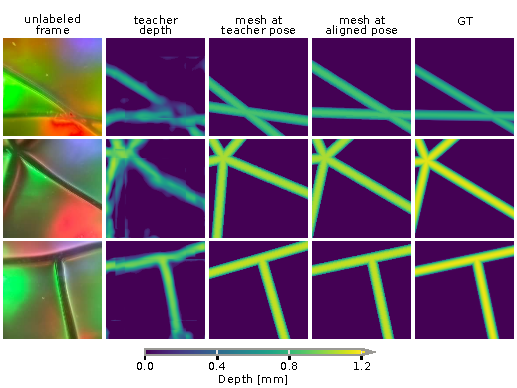
\includegraphics[width=\columnwidth]{figures/fig_align.pdf}
    \caption{\textbf{Pseudo-label construction.} Sensor A, $K=25$. Columns compare teacher depth and mesh projections before and after alignment with GT. Each row is a median-IoU example from a subsampled candidate set for one object. All depth maps use the same scale (mm).}
    \label{fig:align}
\end{figure}

AlignTac converts a small set of registered contacts and a larger pool of unlabeled real images into training data for a tactile predictor. The method first estimates each unlabeled contact state, then projects the known mesh to obtain mutually consistent depth, normal and pose targets.

\noindent\textbf{Geometric labels.} Let $d(\mathcal{M},q)$ denote the depth of object mesh $\mathcal{M}$ at contact state $q=(\theta,x,y,z)$, where $z$ is indentation. For a known object, these variables determine the mesh-derived depth map, its normals and the planar pose. Refinement therefore takes place in contact-state space, with the object geometry held fixed.

\noindent\textbf{Learning the aligner.} A ResNet-18, initialized from ImageNet, takes tactile RGB and candidate mesh depth as four input channels. It predicts a residual $A$ in contact-state units:
\begin{equation}
    \mathcal{A}\big(\mathcal{I},d(\mathcal{M},q^\ast+\delta)\big)\approx-\delta,
\end{equation}
where $q^\ast$ is the labeled state and $\delta$ is a sampled perturbation. The training set is produced by perturbing each registered contact, so learning the correction requires no labels beyond the original $K$ contacts. We normalize the residual dimensions and optimize a smooth-L1 loss; Sec.~\ref{sec:setup} gives the perturbation ranges and training details.

\noindent\textbf{Labeling real images.} For each unlabeled training image, teacher $f_0$ initializes planar pose and sets indentation to its maximum predicted depth. Given the known mesh, we perform six updates,
\begin{equation}
    q_{t+1}=q_t+\mathcal{A}\big(\mathcal{I},d(\mathcal{M},q_t)\big),
\end{equation}
clipping indentation to $[0.3,1.6]\,$mm. The final mesh depth, normals and planar pose label the image. We retain every pseudo-labeled training frame in the evaluated configuration (Sec.~\ref{sec:ablation}).

\noindent\textbf{Training the student.} Student $f_1$ has the teacher's architecture and learns from the $K$ labeled frames and the mesh-aligned frames. Synthetic frames from a renderer may be added as a separate variant; AlignTac itself uses none. Pseudo-labels are generated exclusively from the training split.

\noindent\textbf{Optional test-time refinement.} The student predicts from an image without mesh rendering. When the object identity and mesh are available, the same fixed aligner can refine its predicted pose using the test image. We evaluate this additional inference step separately in Sec.~\ref{sec:tta}.
